\documentclass[12pt,a4paper]{scrartcl} 
\usepackage[utf8]{inputenc}
\usepackage[english,russian]{babel}
\usepackage{indentfirst}
\usepackage{misccorr}
\usepackage{graphicx}
\usepackage{indentfirst}
\usepackage{amsmath}
\begin{document}
	\begin{titlepage}
		\begin{center}
			\large
			МИНИСТЕРСТВО НАУКИ И ВЫСШЕГО ОБРАЗОВАНИЯ РОССИЙСКОЙ ФЕДЕРАЦИИ
			
			Федеральное государственное бюджетное образовательное учреждение высшего образования
			
			\textbf{АДЫГЕЙСКИЙ ГОСУДАРСТВЕННЫЙ УНИВЕРСИТЕТ}
			\vspace{0.25cm}
			
			Инженерно-физический факультет
			
			Кафедра автоматизированных систем обработки информации и управления
			\vfill

			\vfill
			
			\textsc{Отчет по практике}\\[5mm]
			
			{\LARGE Программаная реализация генератора случайных чисел. \LARGE{ Генератор случайных чисел Парка-Миллера с перетасовкой и без.}}
			\bigskip
   
			2 курс, группа 2УТС
		\end{center}
		\vfill
		
		\newlength{\ML}
		\settowidth{\ML}{«\underline{\hspace{0.7cm}}» \underline{\hspace{2cm}}}
		\hfill\begin{minipage}{0.5\textwidth}
			Выполнил:\\
			\underline{\hspace{\ML}} А.\,В.~Сахаутдинов\\
			«\underline{\hspace{0.7cm}}» \underline{\hspace{2cm}} 2020 г.
		\end{minipage}%
		\bigskip
		
		\hfill\begin{minipage}{0.5\textwidth}
			Руководитель:\\
			\underline{\hspace{\ML}} С.\,В.~Теплоухов\\
			«\underline{\hspace{0.7cm}}» \underline{\hspace{2cm}} 2020 г.
		\end{minipage}%
		\vfill
		
		\begin{center}
			Майкоп, 2020 г.
		\end{center}
	\end{titlepage}
	
% Содержание
\section{Введение}
\label{sec:intro}


\subsection{Цель работы}
Целью данной работы является реализация геенератора случайных чисел Парка-Миллера с перетасовкой и без. 

\subsection{Теория}
Самая простая последовательность, которую можно предложить для реализации генератора равномерного распределения:

{\centering(j+1)=a*I(j)(mod m)

}
при соответствующем выборе констант. Константы были предложены Park и Miller:

{\centering a=75=16807, m=231-1=2147483647.

}
Модуль разлагается в выражение:

{\centering m=a*q+r

}
Если r<q и 0<z<m-1, то при этом величины a*(z mod q) и r*[z/q] всегда лежат в интервале 0,...,m-1. Для умножения (a*z)(mod m) при этом используется алгоритм:

    • t = a(z mod q)-r[z/q]

    • если t<0, то t += m.

    • (a*z)(mod m)=t.

В случае констант Парка-Миллера можно использовать q=12773 и r=2836.
\section{Ход работы}
\subsection{Код программы}
\begin{verbatim}
#include <iostream>
#include <vector>
 using namespace std;
 class RandomNumberGenerator
{
   protected:
       unsigned int   init_seed;  // Начальное случайное значение
      unsigned int   cur_seed;   // Текущее случайное значение
      unsigned int   num_draws;  //Размерность
    public:
       RandomNumberGenerator(unsigned int _num_draws,unsigned int _init_seed) :
      num_draws(_num_draws), init_seed(_init_seed), cur_seed(_init_seed)
      {
      };
       virtual ~RandomNumberGenerator()
      {
      };
       virtual unsigned int get_random_seed() const
      {
         return cur_seed;
      }
       virtual void set_random_seed(unsigned int _seed)
      {
         cur_seed = _seed;
      }
   
      virtual void reset_random_seed()
      {
         cur_seed = init_seed;
      }
   
      virtual void set_num_draws(unsigned int _num_draws)
      {
         num_draws = _num_draws;
      }
 
      // получить случайное целое число
      virtual unsigned int  get_random_integer() = 0;
 
      // Заполняет вектор однородными случайными величинами
      //на открытом интервале (0,1)
      virtual void   get_uniform_draws(std::vector<double>& draws) = 0;
};
 
class LinearCongruentialGenerator : public RandomNumberGenerator
{
   private:
      
      double   max_multiplier;
 
   public:
   
LinearCongruentialGenerator(unsigned int _num_draws,unsigned int _init_seed = 1);
virtual ~LinearCongruentialGenerator() 
               {
               };
 
      virtual unsigned int get_random_integer();
      virtual void         get_uniform_draws(std::vector<double>& draws);
};
                     
const unsigned int   a = 16807;       // 7^5
const unsigned int   m = 2147483647;  // 2^32 
 
// Константы алгоритма Шраге
 
const unsigned int   q = 127773;
const unsigned int   r = 2836;
 
// Конструктор параметров
LinearCongruentialGenerator::
LinearCongruentialGenerator(unsigned int _num_draws,unsigned int _init_seed) :
RandomNumberGenerator(_num_draws,_init_seed)
{
   if (!_init_seed)
   {
      init_seed = 1;
      cur_seed  = 1;
   }
 
   max_multiplier = 1.0 / (1.0 + (m - 1));
}
 
// Получает случайное целое число без знака
unsigned int LinearCongruentialGenerator::get_random_integer()
{
   unsigned int   kk  = 0;
 
   kk = cur_seed / q;
   
   cur_seed = a * (cur_seed - kk * q) - r * kk;
 
   if (cur_seed < 0)
   {
      cur_seed += m;
   }
 
   return cur_seed;
}
 // Создайте вектор равномерных участков между (0,1)
void LinearCongruentialGenerator::get_uniform_draws(std::vector<double>& draws)
{
   for (unsigned int ii = 0; ii < num_draws; ++ii)
   {
      draws[ii] = get_random_integer() * max_multiplier;
   }
}
 int main()
{                 
   unsigned int   init_seed = 1;
   unsigned int   num_draws = 20;
    vector<double> random_draws(num_draws,0.0);
    // Cоздать случайные формы
   // открыть интервал (0,1) 
   LinearCongruentialGenerator   lcg(num_draws,init_seed);
    lcg.get_uniform_draws(random_draws);
    // вывод случайных чисел
   for (unsigned int ii = 1; ii < num_draws; ++ii)
   {
      cout << random_draws[ii] << endl;
   }
    system("pause");
    return 0;
}
\end{verbatim}

\begin{figure}[!b]
	\centering
	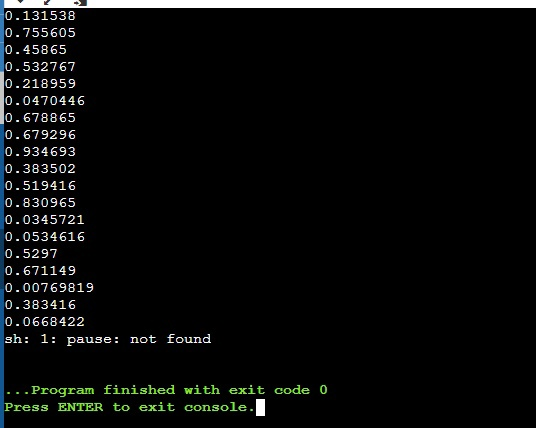
\includegraphics[width=0.7\textwidth]{Рисунок 1.jpg}
	\caption{Окно программы с сгенерированными числами}\label{fig:par}
\end{figure}

\begin{thebibliography}{9}
\bibitem{Knuth-2003}Кнут Д.Э. Всё про \TeX. \newblock --- Москва: Изд. Вильямс, 2003 г. 550~с.
\bibitem{Lvovsky-2003}Львовский С.М. Набор и верстка в системе \LaTeX{}. \newblock --- 3-е издание, исправленное и дополненное, 2003 г.
\bibitem{Voroncov-2005}Воронцов К.В. \LaTeX{} в примерах, 2005 г.
\bibitem{Stroustrup-2013} Страуструп Б. Язык программирования С++, 2013 г.
\bibitem{Koenig-2016} Кёниг Э., Му Б. Эффективное программирование на C++, 2016 г.
\bibitem{Meyers-2018} Мейерс С. Эффективный и современный C++, 2018 г.
\bibitem{Korobkov-2015} Довгаль В.А., Коробков В.Н. Программирование на языке C++ в среде Microsoft Visual Studio --- Часть 1, Учебно-методическое пособие, 2015 г.
\end{thebibliography}

\end{document}
